%!TEX root = ../main.tex

\chapter{Resultados e Discussão} \label{cap:resultados}

Nesta seção serão apresentados os resultados parciais obtidos com o treinamento e teste de algumas arquiteturas canônicas consideradas. A Seção \ref{sec:lenet}  contempla os resultados obtidos com a arquitetura LeNet e a Seção  \ref{sec:alexnet} sintetiza os resultados da arquitetura AlexNet. O treinamento destas CNNs foi realizado utilizando os recursos computacionais de um servidor, disponível no LSI, dedicado especialmente para tarefas de DL, o qual possui um processador Intel Core i7 com 16 GB de RAM e duas placas gráficas com 11 GB de memória cada, das quais apenas uma foi utilizada.

Após a etapa de treino, foram realizados os testes para aferir os modelos no tocante às métricas de desempenho para o conjunto de testes. Nesta etapa, percebeu-se que alguns modelos tornaram-se degenerados e acabaram prevendo apenas uma das classes. Duas hipóteses podem justificar a ocorrência desse problema: o ReLU \emph{dying problem}, quando a função de ativação ReLU foi utilizada; ou a tendência à permanência em mínimos locais durante o treinamento do modelo. Todas as CNNs que manifestaram este comportamento no conjunto de testes tiveram seus resultados descartados, pois as métricas obtidas não refletiam aprendizado no problema considerado.


\section{Resultados Obtidos com a CNN LeNet}
\label{sec:lenet}
%!TEX root = ../../main.tex


A primeira fase do treinamento dos modelos foi conduzida utilizando a arquitetura LeNet. Nesta fase, foi realizada uma busca em \emph{grid} por todos os hiperparâmetros previamente definidos, conforme Seção \ref{sec:modelos}, e considerando as duas abordagens definidas conforme a Seção \ref{sec:preparacao}, gerando um total de $72$ modelos a serem treinados e testados. Para estes modelos, excluindo aqueles que se tornaram degenerados, utilizou-se a métrica \emph{F-Score} como referência para um melhor desempenho.

O melhor dos modelos baseados na arquitetura LeNet para cada uma das abordagens consideradas encontram-se dispostos na Tabela \ref{tab:lenet}, juntamente com os hiperparâmetros utilizados pelos mesmos.

\begin{table}[h]
\centering
\caption{Detalhamento dos melhores resultados obtidos com a arquitetura LeNet.}
\label{tab:lenet}
\resizebox{\textwidth}{!}{\begin{tabular}{ccccccc}
\toprule
\textbf{Abordagem} & \textbf{Otimizador} & \textbf{\emph{Patience}}  & \textbf{Função de Ativação} & \textbf{Acurácia} & \textbf{\emph{F-Score}} & \textbf{EER} \\
\midrule
Abordagem A & RMSprop & 5 & ReLU & $0.9865$ & $0.9755$ & $1.1679$\\
Abordagem B & Adam & 10 & ELU & $0.8361$ & $0.8159$ & $12.5245$ \\
\bottomrule
\end{tabular}}
\end{table}
\todo{Calcular EER para LeNet}


Os gráficos da Figura \ref{fig:treinamento-lenet} denotam o histórico da perda (\emph{loss}) e acurácia para o conjunto de treinamento e validação destas redes. Nota-se que nenhuma delas chegou ao limite máximo de épocas possíveis, interrompendo o aprendizado por meio de \emph{early stopping}, comportamento este que também fez-se presente em todas as outras redes treinadas com esta arquitetura.

\begin{figure}[h!]
	\centering
	\caption{Histórico de \emph{loss} e acurácia durante o treinamento dos melhores modelos obtidos com a arquitetura LeNet.}
	\subfloat[\emph{Loss} durante treinamento da melhor rede LeNet com a abordagem A.\label{subfig:lenet-a-loss}]{%
	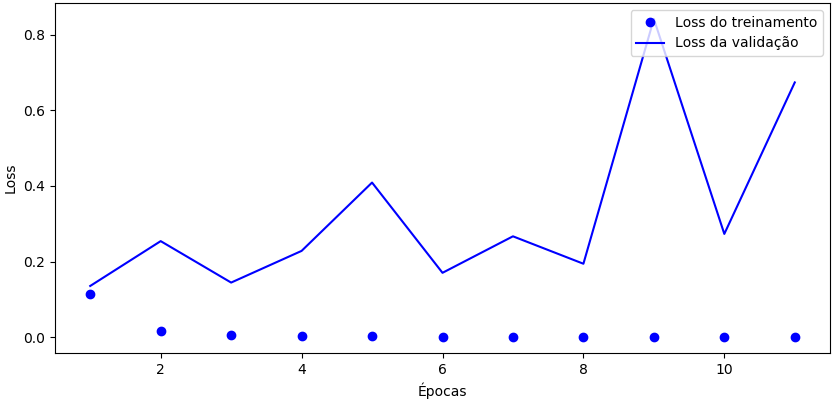
\includegraphics[width=0.45\textwidth]{imgs/lenet-a-loss}
	}
	\hfill
	\subfloat[Acurácia durante treinamento da melhor rede LeNet com a abordagem A.\label{subfig:lenet-a-acc}]{%
	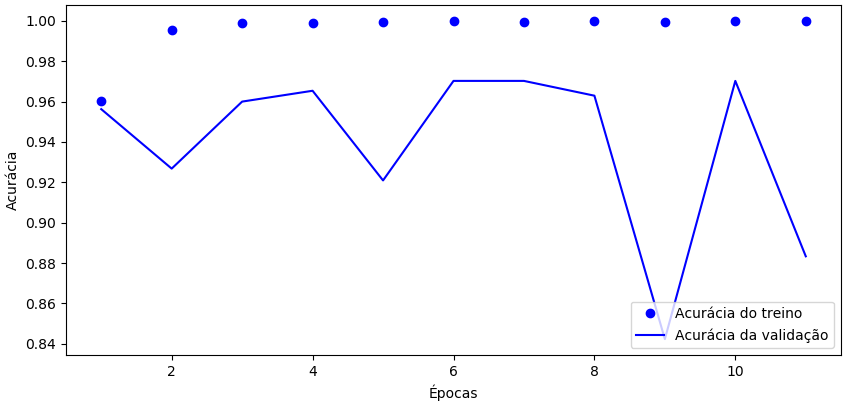
\includegraphics[width=0.45\textwidth]{imgs/lenet-a-acc}
	}
	\hfill
	\subfloat[\emph{Loss} durante treinamento da rede LeNet B.\label{subfig:lenet-b-loss}]{%
	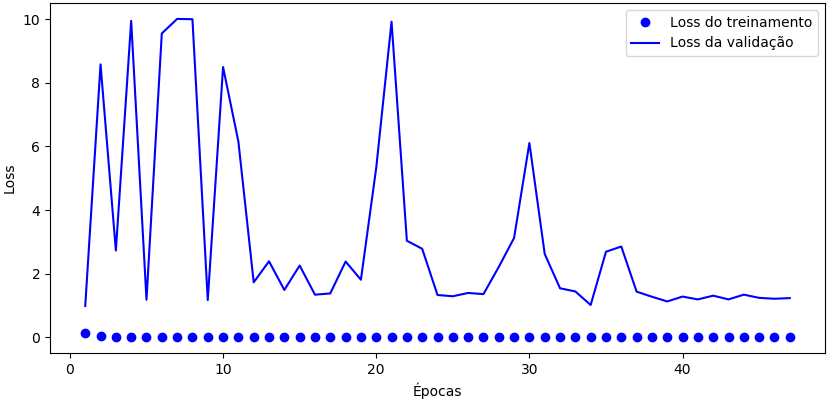
\includegraphics[width=0.45\textwidth]{imgs/lenet-b-loss}
	}
	\hfill
	\subfloat[Acurácia durante treinamento da rede LeNet B.\label{subfig:lenet-b-acc}]{%
	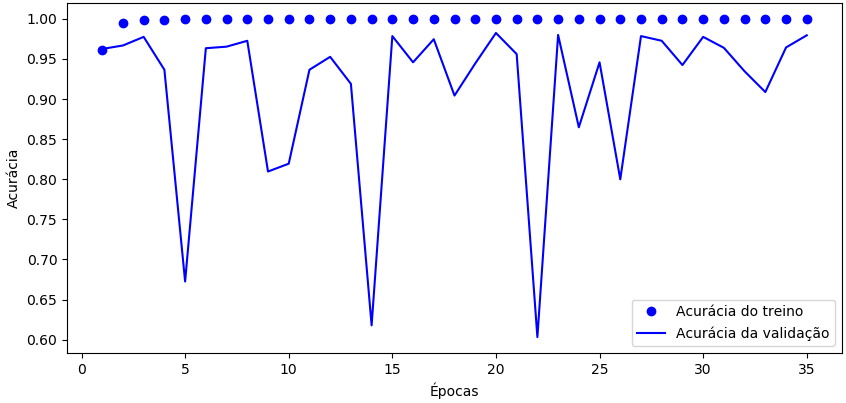
\includegraphics[width=0.45\textwidth]{imgs/lenet-b-acc}
	}
	\label{fig:treinamento-lenet}
\end{figure}

Examinando mais atentamente o desempenho destas redes no conjunto de testes, tem-se, então, as matrizes de confusão mostradas na Figura \ref{fig:matrizes-lenet}. Nestas matrizes, a soma das linhas representam a quantidade de assinaturas previstas para cada classe pelo modelo em questão, enquanto a soma das colunas denotam a quantidade de assinaturas existentes em cada classe.

\begin{figure}[h]
	\centering
	\caption{Matrizes de confusão dos melhores modelos obtidos com a arquitetura LeNet.}\label{fig:matrizes-lenet}
	\subfloat[Melhor LeNet com a abordagem A\label{subfig:matriz-lenet-a}]{%
	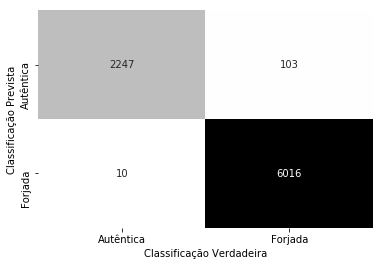
\includegraphics[width=0.47\textwidth]{imgs/matriz-lenet-a}
	}
	\hfill
	\subfloat[Melhor LeNet com a abordagem B\label{subfig:matriz-lenet-b}]{%
	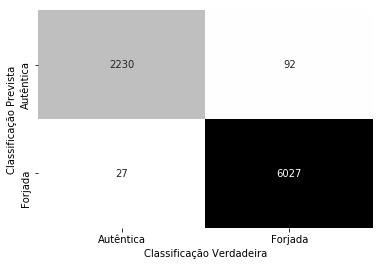
\includegraphics[width=0.47\textwidth]{imgs/matriz-lenet-b}
	}
\end{figure}

%%%% ARGUMENTAÇÃO

Para esta arquitetura, é possível visualizar que, dentre os dois modelos tidos como melhores, não há qualquer semelhança entre os hiperparâmetros encontrados. O número de épocas para aprendizado de características foi baixo para abordagem A, enquanto que, para a abordagem B, houve a necessidade de mais épocas de treinamento. Isso aconteceu, possivelmente, pela aparição de um mesmo autor em partições de dados diferentes na abordagem A.

A partir das matrizes de confusão, percebeu-se que o melhor modelo da abordagem A tendeu a verificar um baixo número de falsos negativos, ou seja, os exemplos autênticos foram suficientes para identificar assinaturas originais, indepentemente das variações cometidas por este autor. Por outro lado, para o modelo da abordagem B, verificou-se um número menor de falsos positivos, validando que, apesar da boa capacidade de certos forjadores \emph{over-the-shoulder} em realizar reproduções verossímeis, este modelo mostrou uma alta competência na detecção deste tipo de assinaturas. Não obstante, nota-se a diagonal principal de ambos os modelos bastante densa, sugerindo uma boa adequação para a tarefa considerada.


\section{Resultados Obtidos com a CNN AlexNet}
\label{sec:alexnet}
%!TEX root = ../../main.tex

%% Trabalhar aqui
Para a AlexNet, assim como para a CNN anterior, foi realizada uma busca em \emph{grid} com os hiperparâmetros selecionados anteriormente, com vistas a obter os melhores modelos para cada abordagem de separação de dados, gerando assim, mais $36$ modelos a serem avaliados quanto às suas métricas de desempenho.

Considerando a métrica de \emph{F-score}, foram selecionados os melhores modelos  desta arquitetura e estes encontram-se listados na Tabela \ref{tab:alexnet}. Na Figura \ref{fig:treinamento-alexnet} pode-se observar os gráficos com os comportamentos dos valores de \emph{loss} e acurácia encontrado nos conjuntos de treinamento e validação durante o estágio de treino destes modelos. Apenas para referência posterior, considerou-se uma rotulação das melhores redes identificadas.

\begin{table}[h!]
\centering
\caption{Detalhamento dos melhores modelos obtidos com a arquitetura AlexNet, organizados de forma decrescente considerando o valor de Acurácia.}
\label{tab:alexnet}
\begin{tabular}{cccccc}
\toprule
\textbf{Identificação} & \textbf{Otimizador} & \textbf{\emph{Patience}}  & \textbf{Função de Ativação} & \textbf{Acurácia} & \textbf{F-Score} \\
\midrule
AlexNet A & Adam & 15 & ELU & $0.9654$ & $0.9393$ \\
AlexNet B & SGD & 10 & \emph{Leaky} ReLU & $0.9601$ & $0.9311$ \\
AlexNet C & SGD & 5 & SELU & $0.9561$ & $0.9244$ \\
\bottomrule
\end{tabular}
\end{table}

\begin{figure}[H]
 \centering
 \caption{Histórico de \emph{loss} e acurácia durante o treinamento dos melhores modelos obtidos com a arquitetura AlexNet.}
 \label{fig:treinamento-alexnet}
 \subfloat[\emph{Loss} durante treinamento da rede AlexNet A.\label{subfig:alexnet-a-loss}]{%
 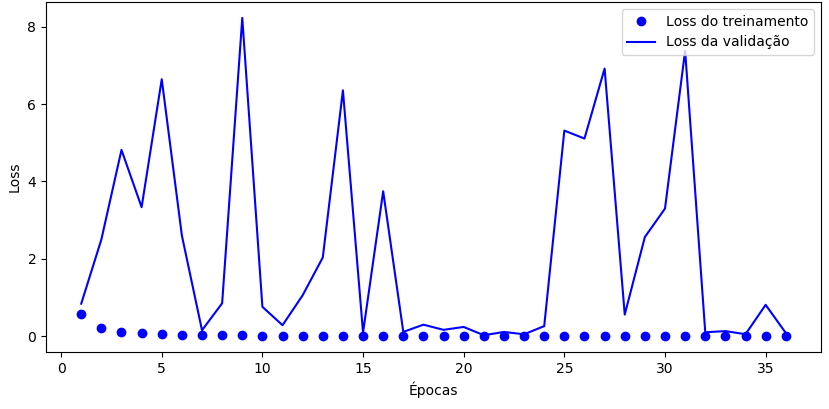
\includegraphics[width=0.45\textwidth]{imgs/alexnet-a-loss}
 }
 \subfloat[Acurácia durante treinamento da rede AlexNet A.\label{subfig:alexnet-a-acc}]{%
 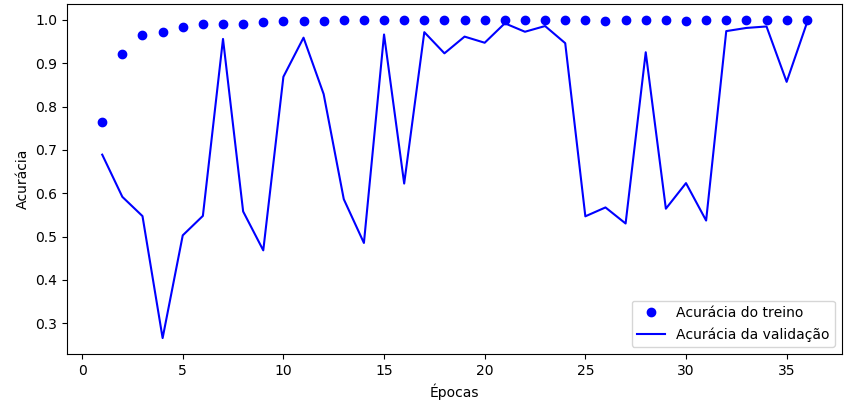
\includegraphics[width=0.45\textwidth]{imgs/alexnet-a-acc}
 }
 \hfill
 \subfloat[\emph{Loss} durante treinamento da rede AlexNet B.\label{subfig:alexnet-b-loss}]{%
 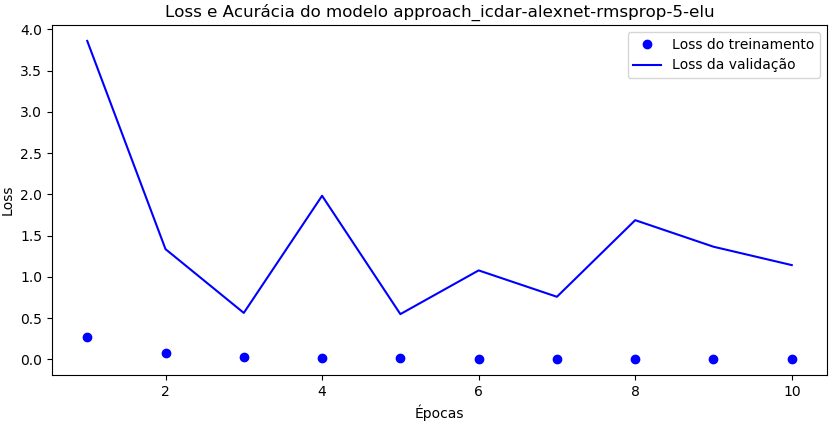
\includegraphics[width=0.45\textwidth]{imgs/alexnet-b-loss}
 }
 \subfloat[Acurácia durante treinamento da rede AlexNet B.\label{subfig:alexnet-b-acc}]{%
 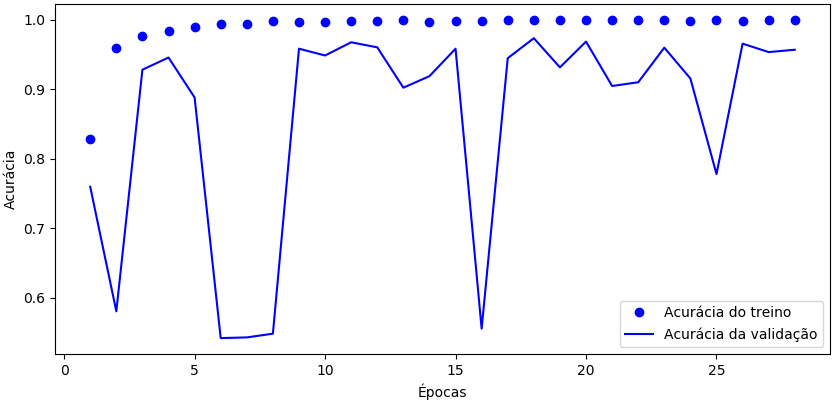
\includegraphics[width=0.45\textwidth]{imgs/alexnet-b-acc}
 }
 \hfill
 \subfloat[\emph{Loss} durante treinamento da rede AlexNet C.\label{subfig:alexnet-c-loss}]{%
 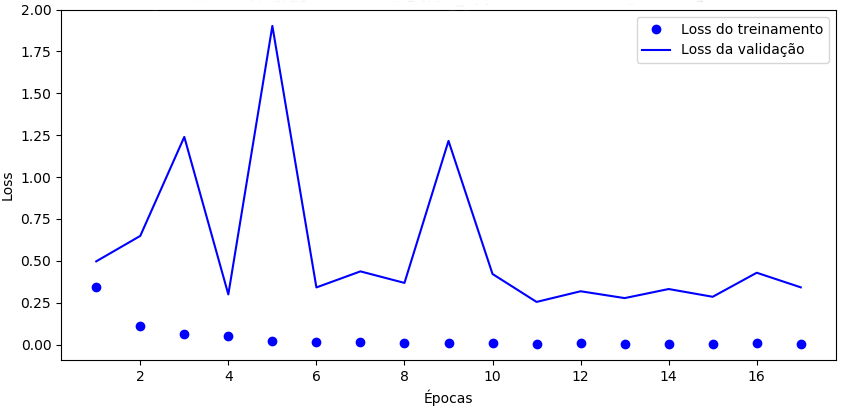
\includegraphics[width=0.45\textwidth]{imgs/alexnet-c-loss}
 }
 \subfloat[Acurácia durante treinamento da rede AlexNet C.\label{subfig:alexnet-c-acc}]{%
 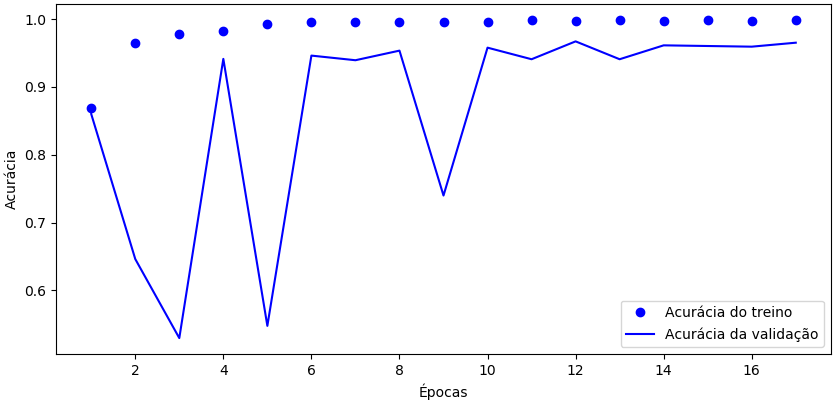
\includegraphics[width=0.45\textwidth]{imgs/alexnet-c-acc}
 }
\end{figure}

Considerando que estas redes possuem mais parâmetros treináveis, este possivelmente foi um fator responsável pelo maior números de épocas no treinamento. Nota-se ainda que houve oscilações nos treinamentos, resultando em parada precoce. Para esta arquitetura, as redes treinadas com otimizador SGD mostraram métricas melhores na etapa de avaliação.

Observando as métricas de acurácia e F-Score obtidas, percebe-se que estas foram inferiores às observadas para as redes LeNet, mas ainda assim alcançando valores superiores a $90\%$. As mesmas reflexões sobre a disposição dos valores na matriz de confusão observados no cenário LeNet se mostram cabíveis, porém com menos acertos.

\begin{figure}[H]
 \centering
 \caption{Matrizes de confusão dos melhores modelos obtidos com a arquitetura AlexNet.}
 \subfloat[AlexNet A\label{subfig:matriz-alexnet-a}]{%
 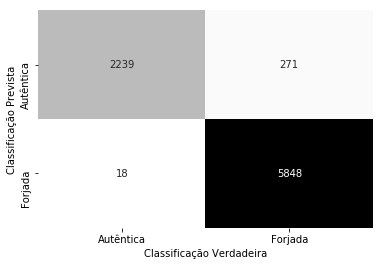
\includegraphics[width=0.5\textwidth]{imgs/matriz-alexnet-a}
 }
 \subfloat[AlexNet B\label{subfig:matriz-alexnet-b}]{%
 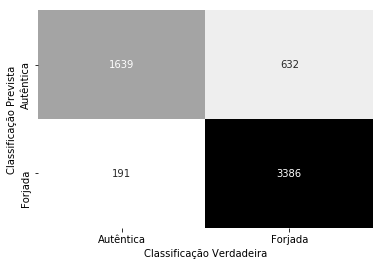
\includegraphics[width=0.5\textwidth]{imgs/matriz-alexnet-b}
 }
 \hfill
 \subfloat[AlexNet C\label{subfig:matriz-alexnet-c}]{%
 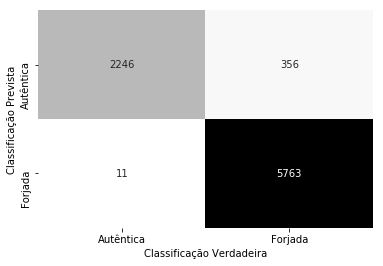
\includegraphics[width=0.5\textwidth]{imgs/matriz-alexnet-c}
 }
 \label{fig:matrizes-alexnet}
\end{figure}

De modo geral, apesar de possuir boas métricas, o melhor modelo encontrado pela arquitetura AlexNet, com um \emph{F-score} de $0.9393$, não foi suficiente para superar o melhor modelo obtido com a arquitetura LeNet ($0.9755$). Uma vez que a arquitetura LeNet possui menos parâmetros que a AlexNet e melhor desempenho observado, ressalta-se a sua maior adequação para a tarefa considerada, acrescido ao fato de demandar menos recursos de tempo de treinamento e de memória para seu armazenamento.

